
\documentclass[letterpaper,hide notes,xcolor={table,svgnames},pdftex,10pt]{beamer}
\def\showexamples{t}

\usecolortheme{crane}
\setbeamertemplate{navigation symbols}{}

\usetheme{MyPittsburgh}
\usepackage{hyperref}
\usepackage{graphicx,xspace}
\usepackage[normalem]{ulem}
\usepackage{multicol}
\usepackage{amsmath,amssymb,amsthm,graphicx,xspace}
\newcommand\SF[1]{$\bigstar$\footnote{SF: #1}}

\usepackage[sfdefault,lf]{carlito}
\usepackage[T1]{fontenc}
\usepackage[scaled]{beramono}
\usepackage{tikzpagenodes}
\newcommand{\Rplus}{\protect\hspace{-.1em}\protect\raisebox{.35ex}{\small{\small\textbf{+}}}}
\newcommand{\Cpp}{\mbox{C\Rplus\Rplus}\xspace}

\newcounter{tmpnumSlide}
\newcounter{tmpnumNote}

\newcommand\mnote[1]{%
	\addtocounter{tmpnumSlide}{1}
	\ifdefined\showcues {~\tiny\fbox{\arabic{tmpnumSlide}}}\fi
	\note{\setlength{\parskip}{1ex}\addtocounter{tmpnumNote}{1}\textbf{\Large \arabic{tmpnumNote}:} {#1\par}}}

\newcommand\mmnote[1]{\note{\setlength{\parskip}{1ex}#1\par}}


\newcommand\mquestion[2]{{~\color{red}\fbox{?}}\note{\setlength{\parskip}{1ex}\par{\Large \textbf{?}} #1} \note{\setlength{\parskip}{1ex}\par{\Large \textbf{A}} #2\par}\ifdefined \presentationonly \pause \fi}

\newcommand\blackboard[1]{%
	\ifdefined   \showblackboard
		{#1}
	\else {\begin{center} \fbox{\colorbox{blue!30}{%
						\begin{minipage}{.95\linewidth}%
							\hspace{\stretch{1}} Some space intentionally left blank; done at the blackboard.%
						\end{minipage}}}\end{center}}%
	\fi%
}

\usepackage{listings}
\lstset{%
	keywordstyle=\bfseries,
	aboveskip=15pt,
	belowskip=15pt,
	captionpos=b,
	identifierstyle=\ttfamily,
	frame=lines,
	numbers=left, basicstyle=\scriptsize, numberstyle=\tiny, stepnumber=0, numbersep=2pt}

\usepackage{siunitx}
\newcommand\sius[1]{\num[group-separator = {,}]{#1}\si{\micro\second}}
\newcommand\sims[1]{\num[group-separator = {,}]{#1}\si{\milli\second}}
\newcommand\sins[1]{\num[group-separator = {,}]{#1}\si{\nano\second}}
\sisetup{group-separator = {,}, group-digits = true}

%% -------------------- tikz --------------------
\usepackage{tikz}
\usetikzlibrary{positioning}
\usetikzlibrary{arrows,backgrounds,automata,decorations.shapes,decorations.pathmorphing,decorations.markings,decorations.text}

\tikzstyle{place}=[circle,draw=blue!50,fill=blue!20,thick, inner sep=0pt,minimum size=6mm]
\tikzstyle{transition}=[rectangle,draw=black!50,fill=black!20,thick, inner sep=0pt,minimum size=4mm]

\tikzstyle{block}=[rectangle,draw=black, thick, inner sep=5pt]
\tikzstyle{bullet}=[circle,draw=black, fill=black, thin, inner sep=2pt]

\tikzstyle{pre}=[<-,shorten <=1pt,>=stealth',semithick]
\tikzstyle{post}=[->,shorten >=1pt,>=stealth',semithick]
\tikzstyle{bi}=[<->,shorten >=1pt,shorten <=1pt, >=stealth',semithick]

\tikzstyle{mut}=[-,>=stealth',semithick]

\tikzstyle{treereset}=[dashed,->, shorten >=1pt,>=stealth',thin]

\usepackage{ifmtarg}
\usepackage{xifthen}
\makeatletter
% new counter to now which frame it is within the sequence
\newcounter{multiframecounter}
% initialize buffer for previously used frame title
\gdef\lastframetitle{\textit{undefined}}
% new environment for a multi-frame
\newenvironment{multiframe}[1][]{%
	\ifthenelse{\isempty{#1}}{%
		% if no frame title was set via optional parameter,
		% only increase sequence counter by 1
		\addtocounter{multiframecounter}{1}%
	}{%
		% new frame title has been provided, thus
		% reset sequence counter to 1 and buffer frame title for later use
		\setcounter{multiframecounter}{1}%
		\gdef\lastframetitle{#1}%
	}%
	% start conventional frame environment and
	% automatically set frame title followed by sequence counter
	\begin{frame}%
		\frametitle{\lastframetitle~{\normalfont(\arabic{multiframecounter})}}%
		}{%
	\end{frame}%
}
\makeatother

\makeatletter
\newdimen\tu@tmpa%
\newdimen\ydiffl%
\newdimen\xdiffl%
\newcommand\ydiff[2]{%
	\coordinate (tmpnamea) at (#1);%
	\coordinate (tmpnameb) at (#2);%
	\pgfextracty{\tu@tmpa}{\pgfpointanchor{tmpnamea}{center}}%
	\pgfextracty{\ydiffl}{\pgfpointanchor{tmpnameb}{center}}%
	\advance\ydiffl by -\tu@tmpa%
}
\newcommand\xdiff[2]{%
	\coordinate (tmpnamea) at (#1);%
	\coordinate (tmpnameb) at (#2);%
	\pgfextractx{\tu@tmpa}{\pgfpointanchor{tmpnamea}{center}}%
	\pgfextractx{\xdiffl}{\pgfpointanchor{tmpnameb}{center}}%
	\advance\xdiffl by -\tu@tmpa%
}
\makeatother
\newcommand{\copyrightbox}[3][r]{%
	\begin{tikzpicture}%
		\node[inner sep=0pt,minimum size=2em](ciimage){#2};
		\usefont{OT1}{phv}{n}{n}\fontsize{4}{4}\selectfont
		\ydiff{ciimage.south}{ciimage.north}
		\xdiff{ciimage.west}{ciimage.east}
		\ifthenelse{\equal{#1}{r}}{%
			\node[inner sep=0pt,right=1ex of ciimage.south east,anchor=north west,rotate=90]%
			{\raggedleft\color{black!50}\parbox{\the\ydiffl}{\raggedright{}#3}};%
		}{%
			\ifthenelse{\equal{#1}{l}}{%
				\node[inner sep=0pt,right=1ex of ciimage.south west,anchor=south west,rotate=90]%
				{\raggedleft\color{black!50}\parbox{\the\ydiffl}{\raggedright{}#3}};%
			}{%
				\node[inner sep=0pt,below=1ex of ciimage.south west,anchor=north west]%
				{\raggedleft\color{black!50}\parbox{\the\xdiffl}{\raggedright{}#3}};%
			}
		}
	\end{tikzpicture}
}


%% --------------------

%\usepackage[excludeor]{everyhook}
%\PushPreHook{par}{\setbox0=\lastbox\llap{MUH}}\box0}

%\vspace*{\stretch{1}

%\setbox0=\lastbox \llap{\textbullet\enskip}\box0}

\setlength{\parskip}{\fill}

\newcommand\noskips{\setlength{\parskip}{1ex}}
\newcommand\doskips{\setlength{\parskip}{\fill}}

\newcommand\xx{\par\vspace*{\stretch{1}}\par}
\newcommand\xxs{\par\vspace*{2ex}\par}
\newcommand\tuple[1]{\langle #1 \rangle}
\newcommand\code[1]{{\sf \footnotesize #1}}
\newcommand\ex[1]{\uline{Example:} \ifdefined \presentationonly \pause \fi
	\ifdefined\showexamples#1\xspace\else{\uline{\hspace*{2cm}}}\fi}

\newcommand\ceil[1]{\lceil #1 \rceil}


\AtBeginSection[]
{
	\begin{frame}
		\frametitle{Outline}
		\tableofcontents[currentsection]
	\end{frame}
}



\pgfdeclarelayer{edgelayer}
\pgfdeclarelayer{nodelayer}
\pgfsetlayers{edgelayer,nodelayer,main}

\tikzstyle{none}=[inner sep=0pt]
\tikzstyle{rn}=[circle,fill=Red,draw=Black,line width=0.8 pt]
\tikzstyle{gn}=[circle,fill=Lime,draw=Black,line width=0.8 pt]
\tikzstyle{yn}=[circle,fill=Yellow,draw=Black,line width=0.8 pt]
\tikzstyle{empty}=[circle,fill=White,draw=Black]
\tikzstyle{bw} = [rectangle, draw, fill=blue!20,
text width=4em, text centered, rounded corners, minimum height=2em]

\newcommand{\CcNote}[1]{% longname
	This work is licensed under the \textit{Creative Commons #1 3.0 License}.%
}
\newcommand{\CcImageBy}[1]{%
	\includegraphics[scale=#1]{creative_commons/cc_by_30.pdf}%
}
\newcommand{\CcImageSa}[1]{%
	\includegraphics[scale=#1]{creative_commons/cc_sa_30.pdf}%
}
\newcommand{\CcImageNc}[1]{%
	\includegraphics[scale=#1]{creative_commons/cc_nc_30.pdf}%
}
\newcommand{\CcGroupBySa}[2]{% zoom, gap
	\CcImageBy{#1}\hspace*{#2}\CcImageNc{#1}\hspace*{#2}\CcImageSa{#1}%
}
\newcommand{\CcLongnameByNcSa}{Attribution-NonCommercial-ShareAlike}

\newenvironment{changemargin}[1]{% 
	\begin{list}{}{% 
		\setlength{\topsep}{0pt}% 
		\setlength{\leftmargin}{#1}% 
		\setlength{\rightmargin}{1em}
		\setlength{\listparindent}{\parindent}% 
		\setlength{\itemindent}{\parindent}% 
		      \setlength{\parsep}{\parskip}% 
		      }% 
		\item[]}{\end{list}}




\title{Lecture 7 --- Stack Management }

\author{Jeff Zarnett \& Mike Cooper-Stachowsky \\ \small \texttt{jzarnett@uwaterloo.ca, mstachowsky@uwaterloo.ca}}
\institute{Department of Electrical and Computer Engineering \\
  University of Waterloo}
\date{\today}


\begin{document}

\begin{frame}
	\titlepage

\end{frame}


\begin{frame}
\frametitle{So You Want To Manage a Stack}

Stack management is a challenging but important subject.

\begin{center}
	
\includegraphics[width=0.5\textwidth]{images/herosquest.png}
\end{center}

Goals: learn about the stack, the Cortex M's stack pointers, and the Application-Binary Interface.


\end{frame}


\begin{frame}
\frametitle{What Goes on the Stack?}

1. Local variables

2. Context variables: function args, return addresses...

3. Register data or other state storage

\end{frame}


\begin{frame}
\frametitle{FIFO Behaviour}

Remember that the stack is a FIFO data structure:

\alert{Push} things on to the stack...

\alert{Pop} things off of the stack...

Cannot remove things from the middle...\\
\quad But I mean, it's just memory, so you \textit{can} do bad things... but shouldn't.


\end{frame}



\begin{frame}[fragile]
\frametitle{Function Call With Annotations}

\begin{lstlisting}[language=C]
int do_something( int x ) {
  if ( x > 30 ) {
    int y = 5;
    return y+x;
  }
  return x - 10;
}
\end{lstlisting}

\begin{itemize}
	\item PUSH return address (but not \texttt{x})
	\item If \texttt{x > 30}
		\begin{itemize}
			\item Push \texttt{y}
			\item Add \texttt{y + x}
			\item Put result into Register \texttt{R0}
			\item POP \texttt{y}
			\item JUMP to return address
			\item POP return address
		\end{itemize}
	\item Otherwise:
		\begin{itemize}
		\item Compute \texttt{x - 10}
		\item Put the result into Register \texttt{R0}
		\item JUMP to return address
		\item POP return address
	\end{itemize}
\end{itemize}


\end{frame}


\begin{frame}
\frametitle{Function Call with Annotation}

\begin{center}
	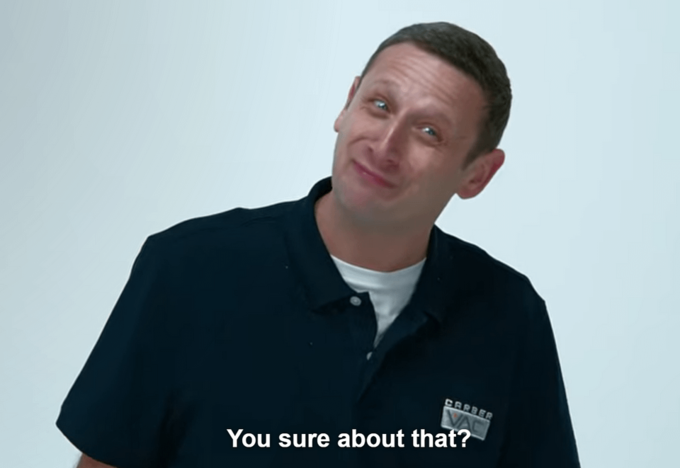
\includegraphics[width=0.4\textwidth]{images/sureaboutthat.png}
\end{center}

Some things in that list are a bit suspect. Why?

\end{frame}


\begin{frame}
\frametitle{Location, Location, and Optimization}

The compiler optimizes! Remove \texttt{int y = 5;} and make it \texttt{return 5 + x}

	
Computations need memory locations so instead of adding \texttt{5 + x} somewhere else and then putting it into \texttt{R0}, make that the destination.

So the branch of \texttt{x > 30} probably looks more like:
\begin{itemize}
	\item LOAD \texttt{x} into \texttt{R0}
	\item \texttt{R0 = R0 + 5}
	\item JUMP to return address
	\item POP return address
\end{itemize}

\end{frame}


\begin{frame}
\frametitle{But Did It Work?}

The example still gives us some idea about pushing and popping from the stack.

Every thread-local variable will have a stack location or a register.

When the function ends, everything  from that function is popped off the stack. 

\end{frame}


\begin{frame}
\frametitle{In Balance}

PUSH and POP operations must be equal. 

\begin{center}
	
\includegraphics[width=0.5\textwidth]{images/balance-force.jpg}
\end{center}

So no have memory leaks, though we can run out of space (overflow).

\end{frame}


\begin{frame}
\frametitle{Stacks Grow Where?}

Typically we think of a stack like its physical representation.

Software stacks may grow down rather than up.\\
\quad So PUSH decrements the stack pointer and POP increments it.

If the stack is empty and we push data: write it, decrement SP.\\
\quad If it's not empty (``full''), decrement SP then write.

\end{frame}



\begin{frame}
\frametitle{Cortex M4 Stack Organization}

\texttt{SP}: ``The'' stack pointer, used by the processor to access the stack.

\texttt{MSP}: ``Main'' stack pointer, always used in interrupts, initialized via reset vector address \texttt{0x0}.

\texttt{PSP}: ``Process'' stack pointer, never used in interrupts, initialized by user/programmer.


\end{frame}


\begin{frame}
\frametitle{Too Many of Them?}

\begin{center}
	
\includegraphics[width=0.5\textwidth]{images/sptdh.jpg}
\end{center}

SP is directly connected to the CPU (need it).

PSP can never be used by privileged code; MSP is for privileged code.

\end{frame}


\begin{frame}
\frametitle{Let's Get Started}

At boot time SP is probably 0 (not good).

At load time memory segments get set up.

The vector reset table is used (see next slide).

The initial value of the MSP (SP) is \texttt{0x0}...\\
\quad Access it as: \texttt{uint32\_t* MSP\_INIT = *(uint32\_t*) 0;}

\end{frame}



\begin{frame}
\frametitle{Reset Vector Table}

\begin{center}
	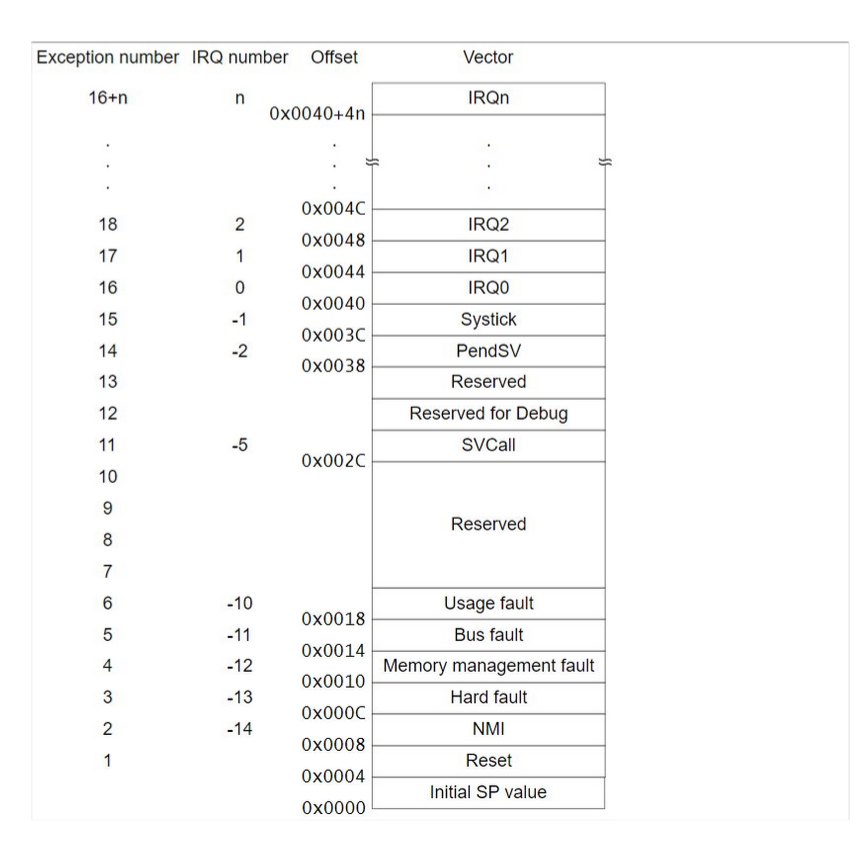
\includegraphics[width=0.7\textwidth]{images/rvtable.png}
\end{center}

\end{frame}


\begin{frame}
\frametitle{Application Binary Interface}

The ABI is rules developed by chip designers for compilers to know.

\begin{center}
	
\includegraphics[width=0.3\textwidth]{images/thelaw.jpg}
\end{center}

We'll look at the stack rules, but there's more complexity we're skipping.

ABI says the stack is full and descending.\\
\quad Any other organization is not following the rules.

\end{frame}


\begin{frame}
\frametitle{Passing Arguments}

Registers \texttt{R0 - R3} are the ``argument'' and ``result'' registers.\\
\quad Precisely \texttt{4x4} bytes of space for arguments.

Each register is one of:\\\begin{itemize}
	\item A 4-byte type (e.g., \texttt{uint\_32})
	\item A smaller-than-4-byte type (space is wasted)
	\item A portion of a larger type (e.g., half of a \texttt{uint\_64}
\end{itemize}


Registers fill from \texttt{R0} to \texttt{R3}.


\end{frame}


\begin{frame}[fragile]
\frametitle{Argument Examples}

\begin{lstlisting}[language=C]
uint_32 a, b;
uint_64 c, d, e;

/* Initialization not shown */

foo( a, b ); // a goes in R0, b goes in R1


bar( a, b, c ); // a goes in R0, b in R1, c is split over R2 and R3.


big_fun( a, b, c, d, e ); // Where do they go?

\end{lstlisting}


\end{frame}


\begin{frame}[fragile]
\frametitle{Argument Examples}

\begin{lstlisting}[language=C]
uint_32 a, b;
uint_64 c, d, e;

/* Initialization not shown */

foo( a, b ); // a goes in R0, b goes in R1


bar( a, b, c ); // a goes in R0, b in R1, c is split over R2 and R3.


big_fun( a, b, c, d, e ); // Where do they go?

\end{lstlisting}

You guessed it: additional function arguments go on the stack!

The compiler may need to add code to shuffle them around.

\end{frame}


\begin{frame}[fragile]
\frametitle{Is it Useful?}

If the compiler is going to do it, do we need to know about it?

Yes, if we're going to call a C function from assembly!

\begin{verbatim}
MOV R0, #3
MOV R1, #4
BL foo
\end{verbatim}

The above is equivalent to calling \texttt{foo( 3, 4 );}

\end{frame}


\begin{frame}[fragile]
\frametitle{Chained Function Calls}

\begin{lstlisting}[language=C]
int f1( int x, int y ) {
  return x + y;
}

int f2( int a, int b, int c ) {
  int x = f1( 3, 4 );
  return x + a + b + c;
}
\end{lstlisting}


Can't put 3 and 4 in \texttt{R0, R1} because they contain \texttt{a, b} that we still need.

Now what? 

\end{frame}


\begin{frame}
\frametitle{Compiler!}

\begin{center}
	
\includegraphics[width=0.4\textwidth]{images/NoProblemo.png}
\end{center}

In this specific example the compiler can just replace the call to \texttt{f1} with the add operation and change the return statement to be: \texttt{return 7 + a + b + c}.

But suppose it did not or could not do that?

\end{frame}


\begin{frame}
\frametitle{Write it Down!}

Solution is hardware saved registers!

\texttt{R0 - R3, PC, LR, SP} are pushed onto the stack by the hardware.\\
\quad So the compiler does not have to do this.

This is part of the ``call stack'' that helps us trace how we got here.

When a function ends, those values are popped \& put back where they were.
\end{frame}


\begin{frame}
\frametitle{Other Registers?}

Other registers \texttt{R4 - R11} are called \alert{scratch}.

We don't have to preserve them across function calls.

It will be our responsibility to store/restore them when switching between threads (context switch, scheduling).

The compiler doesn't manage them and things can change.

\end{frame}



\begin{frame}
\frametitle{Return Values}

Any data type less than 4 bytes goes into \texttt{R0}.

Anything bigger than 4 bytes but less than 16 is spread over the needed amount of \texttt{R0-R3}, like the input arguments.

After that, the compiler will put it elsewhere and return a pointer in \texttt{R0}.


\end{frame}



\end{document}

